\section{Formation des jets}\label{chapter-JERC-section-jets}
Lorsqu'une particule colorée, \ie\ un quark ou un gluon, est issue de la collision, cette particule possède une haute énergie et $g_s \ll 1$. Cette particule colorée radie, par interaction forte, d'autres particules colorées. Par conservation, l'énergie portée portée par chaque particule colorée ainsi obtenue diminue et par conséquence, $g_s$ augmente.
\par Tant que l'échelle d'énergie est suffisamment grande pour que $g_s \ll 1$, ce qui correspond à des énergies supérieures à la centaine de \SI{}{\MeV}, il est possible de réaliser des calculs perturbatifs. La radiation de particules colorées créé ce que s'appelle la \og gerbe partonique \fg, ce qui est le sujet de la prochaine section.
\par Au fur et à mesure des radiations, l'échelle en énergie diminue et en deçà d'une centaine de \SI{}{\MeV}, il n'est plus possible de réaliser des calculs perturbatifs car $g_s$ augmente. Des modèles paramétriques sont alors utilisés pour caractériser le phénomène de \og hadronisation \fg, sujet de la section suivante.

\subsection{Gerbe partonique}\label{chapter-JERC-section-jets-subsec-gerbe-partonique}
%\fullcite{Unorthodox_Introduction_QCD}
Lorsqu'une particule colorée est issue d'une collision au LHC, elle se trouve dans un premier temps dans le régime de liberté asymptotique. Elle radie alors d'autres particules colorées. Ainsi, pour un événement $\Zboson\to\quark\antiquark$ comme celui de la figure~\ref{subfig-fgraph-Z_q_q} avec deux quarks dans l'état final, il est possible d'obtenir par radiation d'un gluon un état $\quark\antiquark\gluon$ comme ceux illustrés sur les figures~\ref{subfig-fgraph-Z_qg_q} et~\ref{subfig-fgraph-Z_q_qg}, par exemple.
\begin{figure}[h]
\centering\vspace{\baselineskip}
\subcaptionbox{\label{subfig-fgraph-Z_q_q}}[.3\textwidth]
{\begin{fmffile}{Z_q_q}\fmfstraight
\begin{fmfchar*}(30,20)
  \fmfleft{i}
  \fmfright{o1,o3}
  \fmf{boson, tension=2}{i,v1}
  \fmf{phantom}{o1,v1,o3}
  \fmffreeze
  \fmf{fermion}{o1,v1,o3}
  \fmflabel{\Zboson}{i}
  \fmflabel{\quark}{o3}
  \fmflabel{\antiquark}{o1}
  \fmfdot{v1}
\end{fmfchar*}
\end{fmffile}
\vspace{\baselineskip}}
\hfill
\subcaptionbox{\label{subfig-fgraph-Z_qg_q}}[.3\textwidth]
{\begin{fmffile}{Z_qq_q}\fmfstraight
\begin{fmfchar*}(30,20)
  \fmfleft{i}
  \fmfright{o1,o2,o0,o3}
  \fmf{boson, tension=2}{i,v1}
  \fmf{phantom}{o1,v1,o3}
  \fmffreeze
  \fmf{fermion}{o1,v2,v1,o3}
  \fmffreeze
  \fmf{gluon}{v2,o2}
  \fmflabel{\gluon}{o2}
  \fmflabel{\Zboson}{i}
  \fmflabel{\quark}{o3}
  \fmflabel{\antiquark}{o1}
  \fmfdot{v1,v2}
\end{fmfchar*}
\end{fmffile}
\vspace{\baselineskip}}
\hfill
\subcaptionbox{\label{subfig-fgraph-Z_q_qg}}[.3\textwidth]
{\input{\PhDthesisdir/tex/Feynman_diagrams/gerbe_partonique/fgraph-Z_q_qg.tex}\vspace{\baselineskip}}
\caption{Un boson \Zboson\ se désintègre en paire quark-antiquark. Dans les cas des figures~\ref{subfig-fgraph-Z_qg_q} et~\ref{subfig-fgraph-Z_q_qg}, un gluon supplémentaire est radié.}
\label{fig-fgraph-Z_q_q_xg}
\end{figure}
\par Il est légitime de se demander quelle est la probabilité d'obtenir un état $\quark\antiquark\gluon$ à partir d'un état $\quark\antiquark$.
Des calculs de section efficace permettent d'obtenir~\cite{salam2010elements}, pour un état initialement à $X$ partons dont un parton $i$ radie un parton $j$,
\begin{equation}
\dd{\sigma_{X+j}} \simeq \sigma_{X} \sum_{i\in\set{X}} \frac{g_s}{2\pi} \frac{\dd{\theta^2}}{\theta^2} \dd{z} P_{ij}(z)
\end{equation}
où $\theta$ est l'angle entre le parton radié $j$ et le parton radiant $i$. La grandeur $P_{ij}(z)$ est la probabilité qu'un parton de type $i$ radie un parton de type $j$ emportant une fraction $z$ de l'énergie initiale de $i$, qui s'exprime
\begin{align}
P_{\quark\quark}(z) &= C_F \frac{1+z^2}{1-z} \msep&
P_{\quark\gluon}(z) &= C_F \frac{1+(1-z)^2}{z} \mend[,]
\\
P_{\gluon\gluon}(z) &= C_A \frac{z^4 + 1 + (1-z)^4}{z(1-z)} \msep&
P_{\gluon\quark}(z) &= T_R (z^2+(1-z)^2) \mend[,]
\end{align}
et $P_{\gluon\antiquark}(z) = P_{\gluon\quark}(z)$,
avec
$C_F=\frac{4}{3}$,
$C_A = 3$ et
$T_R=\frac{1}{2}$.
La probabilité de radier un parton supplémentaire diverge dans deux cas:
\begin{itemize}
\item le parton rayonné a une énergie faible devant celle du parton rayonnant, c'est la limite infrarouge;
\item l'angle entre le parton rayonné est le parton rayonnant est petit, c'est la limite colinéaire.
\end{itemize}
\par Les nouveaux partons ainsi radiés, et les partons initiaux, continuent chacun ce processus jusqu'à ce que le phénomène de confinement de couleur réapparaisse. Nous obtenons alors, pour un parton directement issu de la collision, une gerbe partonique, \ie\ un ensemble collimé de particules colorées, ce qui est illustré sur la figure~\ref{fig-parton_shower}.
Ce sont ces particules qui vont participer au phénomène de hadronisation dû au confinement de couleur.
\begin{figure}[h]
\centering
\subcaptionbox{Deux quarks sont initialement produits, ce qui correspond au diagramme de la figure~\ref{subfig-fgraph-Z_q_q}.\label{subfig-parton_shower-qq}}[.32\textwidth]
{\begin{tikzpicture}
\def\Lenght{2.5}
\def\qangle{45}
\def\antiqangle{\qangle+180}

\clip (-\Lenght,-\Lenght) rectangle (\Lenght,\Lenght) ;

\fill (0,0) circle (2pt);
\draw (0,0) node [left] {PV} ;

\draw (0,0) --+ (\qangle:\Lenght) node [left] {\quark} ;
\draw (0,0) --+ (\antiqangle:\Lenght) node [right] {\antiquark} ;


\end{tikzpicture}}
\hfill
\subcaptionbox{Un des quarks peut radier un gluon, ce qui correspond au diagramme de la figure~\ref{subfig-fgraph-Z_q_qg}.\label{subfig-parton_shower-qqg}}[.32\textwidth]
{\begin{tikzpicture}
\def\Lenght{2.5}
\def\qangle{45}
\def\antiqangle{\qangle+180}

\clip (-\Lenght,-\Lenght) rectangle (\Lenght,\Lenght) ;

\fill (0,0) circle (2pt);
\draw (0,0) node [left] {PV} ;

\draw (0,0) --+ (\qangle:\Lenght) node [left] {\quark} ;
\draw (0,0) --+ (\antiqangle:\Lenght) node [right] {\antiquark} ;


\def\Lfrac{3}
\draw (0,0) --+ (\qangle:\Lenght/\Lfrac) coordinate (g1) ;
\draw (g1) + (\qangle-30:\Lenght-\Lenght/\Lfrac) coordinate (g2) ;
\draw [decoration={aspect=0.6, segment length=1.75mm, amplitude=1mm,coil},decorate] (g2) -- (g1) ;

\end{tikzpicture}}
\hfill
\subcaptionbox{Le processus est réitéré, donnant un ensemble de particules colorées.\label{subfig-parton_shower-qqNg}}[.32\textwidth]
{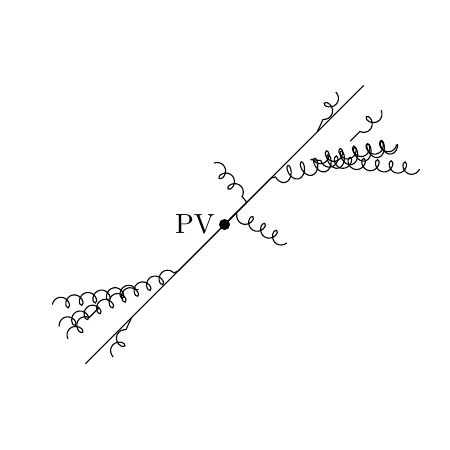
\begin{tikzpicture}
\def\Lenght{2.5}
\def\qangle{45}
\def\antiqangle{\qangle+180}

\clip (-\Lenght,-\Lenght) rectangle (\Lenght,\Lenght) ;

\fill (0,0) circle (2pt);
\draw (0,0) node [left] {PV} ;

\draw (0,0) --+ (\qangle:\Lenght) node [left] {\quark} ;
\draw (0,0) --+ (\antiqangle:\Lenght) node [right] {\antiquark} ;


\def\Lfrac{3}
\draw (0,0) --+ (\qangle:\Lenght/\Lfrac) coordinate (g1) ;
\draw (g1) + (\qangle-30:\Lenght-\Lenght/\Lfrac) coordinate (g2) ;
\draw [decoration={aspect=0.6, segment length=1.75mm, amplitude=1mm,coil},decorate] (g2) -- (g1) ;

\draw (g1) + (\qangle-20:{(\Lenght-\Lenght/\Lfrac)/(\Lfrac/2)}) coordinate (g3) ;
\draw (g3) + (\qangle:{\Lenght-\Lenght/\Lfrac-(\Lenght-\Lenght/\Lfrac)/(\Lfrac/2)}) coordinate (g4) ;
\draw [decoration={aspect=0.8, segment length=1.75mm, amplitude=.75mm,coil},decorate] (g4) -- (g3) ;

\draw (g1) + (\qangle-20:{(\Lenght-\Lenght/\Lfrac)/(\Lfrac)}) coordinate (g3) ;
\draw (g3) + (\qangle-35:{\Lenght-\Lenght/\Lfrac-(\Lenght-\Lenght/\Lfrac)/(\Lfrac)}) coordinate (g4) ;
\draw [decoration={aspect=0.8, segment length=1.75mm, amplitude=.75mm,coil},decorate] (g4) -- (g3) ;

\draw (g3) + (\qangle-50:{\Lenght-\Lenght/\Lfrac-(\Lenght-\Lenght/\Lfrac)/(\Lfrac*2)}) coordinate (g4) ;
\draw [decoration={aspect=0.8, segment length=1.75mm, amplitude=.75mm,coil},decorate] (g4) -- (g3) ;

\draw (g1) + (\qangle:{(\Lenght-\Lenght/\Lfrac)/(2*\Lfrac/3)}) coordinate (g3) ;
\draw (g3) + (\qangle+20:{\Lenght-\Lenght/\Lfrac-(\Lenght-\Lenght/\Lfrac)/(\Lfrac/2)}) coordinate (g4) ;
\draw [decoration={aspect=0.8, segment length=1.75mm, amplitude=.75mm,coil},decorate] (g4) -- (g3) ;

%% qbar shower
\draw (0,0) --+ (\antiqangle:\Lenght/\Lfrac) coordinate (g1) ;
\draw (g1) + (\antiqangle-20:\Lenght-\Lenght/\Lfrac) coordinate (g2) ;
\draw [decoration={aspect=0.8, segment length=1.75mm, amplitude=.75mm,coil},decorate] (g2) -- (g1) ;

\draw (g1) + (\antiqangle-20:{(\Lenght-\Lenght/\Lfrac)/(\Lfrac/2)}) coordinate (g3) ;
\draw (g3) + (\antiqangle:{\Lenght-\Lenght/\Lfrac-(\Lenght-\Lenght/\Lfrac)/(\Lfrac/2)}) coordinate (g4) ;
\draw [decoration={aspect=0.8, segment length=1.75mm, amplitude=.75mm,coil},decorate] (g4) -- (g3) ;

\draw (g1) + (\antiqangle-20:{(\Lenght-\Lenght/\Lfrac)/(\Lfrac)}) coordinate (g3) ;
\draw (g3) + (\antiqangle-35:{\Lenght-\Lenght/\Lfrac-(\Lenght-\Lenght/\Lfrac)/(\Lfrac)}) coordinate (g4) ;
\draw [decoration={aspect=0.8, segment length=1.75mm, amplitude=.75mm,coil},decorate] (g4) -- (g3) ;

%\draw (g3) + (\antiqangle-50:{\Lenght-\Lenght/\Lfrac-(\Lenght-\Lenght/\Lfrac)/(\Lfrac*2)}) coordinate (g4) ;
%\draw [decoration={aspect=0.8, segment length=1.75mm, amplitude=.75mm,coil},decorate] (g4) -- (g3) ;

\draw (g1) + (\antiqangle:{(\Lenght-\Lenght/\Lfrac)/(2*\Lfrac/3)}) coordinate (g3) ;
\draw (g3) + (\antiqangle+20:{\Lenght-\Lenght/\Lfrac-(\Lenght-\Lenght/\Lfrac)/(\Lfrac/2)}) coordinate (g4) ;
\draw [decoration={aspect=0.8, segment length=1.75mm, amplitude=.75mm,coil},decorate] (g4) -- (g3) ;

%% soft gluons
\draw (0,0) --+ (\qangle:.2) coordinate (g1) ;
\draw (g1) + (\qangle-75:.75) coordinate (g2) ;
\draw [decoration={aspect=0.8, segment length=1.75mm, amplitude=.75mm,coil},decorate] (g2) -- (g1) ;

\draw (0,0) --+ (\qangle:.4) coordinate (g1) ;
\draw (g1) + (\qangle+85:.65) coordinate (g2) ;
\draw [decoration={aspect=0.8, segment length=1.75mm, amplitude=.75mm,coil},decorate] (g2) -- (g1) ;

\end{tikzpicture}}

\caption{Illustration de la formation de deux gerbes partoniques à partir d'une paire de quarks.}
\label{fig-parton_shower}
\end{figure}

\subsection{Hadronisation}\label{chapter-JERC-section-jets-subsec-hadronisation}

% \PhDthesisdir/tex/Feynman_diagrams/QCD/fgraph-QCD_clustering_fragmentation.tex

cordes de Lund\footcite{Andersson_parton_fragmentation}

agglomération hadronique\footcite{Winter_2004}
